\documentclass[a4paper,12pt]{report}

\usepackage[vietnamese]{babel}
\usepackage[utf8]{inputenc, vietnam}
\usepackage[a4paper,margin=24mm]{geometry}
\usepackage[skip=10pt plus1pt, indent=20pt]{parskip}
\usepackage[colorlinks=true,allcolors=blue,urlcolor=magenta]{hyperref}

\usepackage{caption}
\usepackage{indentfirst,setspace,subcaption}
\usepackage{amsmath,amssymb,graphicx,xcolor,url}
\usepackage{fancyhdr,tocbasic,titlesec,minted,listings}

\renewcommand{\thesection}{\arabic{section}}

% Header and footer styling
\pagestyle{fancy}
\setlength{\headheight}{18pt}
\fancyhf{}
\fancyhead[R]{\nouppercase\rightmark\hfill~Báo cáo bài tập 2}
\fancyfoot[C]{\hfill\thepage\hfill}

% TOC styling
\DeclareTOCStyleEntry[
  indent=12pt,
  level=1
]{largetocline}{section}

% Title page data
\title{Báo cáo bài tập 2}
\author{\begin{tabular}{r c}
  Ngô Nguyễn Thế Khoa & 23127065
  \end{tabular}}
\date{Ngày 21 tháng 10 năm 2024}

\begin{document}

% Title page and TOC
\thispagestyle{empty}
\begin{titlepage}
	\begin{center}
		\makeatletter
		\newcommand{\HRule}{\rule{\linewidth}{0.4mm}}

		\textsc{\LARGE Vietnam National University,\\Ho Chi Minh City}\\[1.5cm]
		\textsc{\Large University of Science}\\[0.5cm]
		\textsc{\Large Faculty of Information Technology}\\[1.5cm]

		{\HRule}\\[1cm]
		{\huge \bfseries \@title}\\[0.5cm]
		{\HRule}\\[2cm]

		\textsc{\large CSC10004 -- Data Structures and Algorithms}\\[0.5cm]

		\vfill\vfill\vfill

		{\large \@author}\\[1.5cm]
		{\large \@date}
		\makeatother
	\end{center}
\end{titlepage}
\tableofcontents\thispagestyle{empty}

% Report contents
\pagebreak
\section{Đánh giá}
\subsection*{Bảng đánh giá mức độ hoàn thành}
\begin{center}
	\renewcommand{\arraystretch}{1.5}
	\begin{tabular}{|c|p{\dimexpr0.7\linewidth-\tabcolsep}|c|}
		\hline
		\textbf{STT} & \textbf{Yêu cầu}                                                                                                                           & \textbf{Tiến độ} \\\hline
		\multicolumn{3}{|c|}{\textbf{Bài tập 1}}                                                                                                                                     \\\hline
		1            & Viết chương trình nhập vào số chấm động. Hãy xuất ra biểu diễn nhị phân từng thành phần (dấu, phần mũ, phần trị) của số chấm động vừa nhập & 100\%            \\\hline
		\multicolumn{3}{|c|}{\textbf{Bài tập 2}}                                                                                                                                     \\\hline
		1            & Viết chương trình nhập vào biểu diễn nhị phân của số chấm động. Hãy xuất ra biểu diễn thập phân tương ứng                                  & 100\%            \\\hline
		\multicolumn{3}{|c|}{\textbf{Bài tập 3}}                                                                                                                                     \\\hline
		1            & 1.3E+20 có biểu diễn nhị phân ra sao                                                                                                       & 100\%            \\\hline
		2            & Số float nhỏ nhất lớn hơn 0 là số nào? Biểu diễn nhị phân của nó?                                                                          & 100\%            \\\hline
		3            & Những trường hợp nào tạo ra các số đặc biệt (kiểu float) (viết chương trình thử nghiệm và giải thích kết quả)                              & 100\%            \\\hline
		\multicolumn{3}{|c|}{\textbf{Bài tập 4}}                                                                                                                                     \\\hline
		1            & Chuyển đổi float -> int -> float. Kết quả như ban đầu?                                                                                     & 100\%            \\\hline
		2            & Chuyển đổi int -> float -> int. Kết quả như ban đầu?                                                                                       & 100\%            \\\hline
		3            & Phép cộng số chấm động có tính kết hợp?                                                                                                    & 100\%            \\\hline
		4            & \verb|i = (int) (3.14159 * f);|                                                                                                            & 100\%            \\\hline
		5            & \verb|f = f + (float) i;|                                                                                                                  & 100\%            \\\hline
		6            & \verb|if (i == (int)((float) i)) { printf(“true”); }|                                                                                      & 100\%            \\\hline
		7            & \verb|if (i == (int)((double) i)) { printf(“true”); }|                                                                                     & 100\%            \\\hline
		8            & \verb|if (f == (float)((int) f)) { printf(“true”); }|                                                                                      & 100\%            \\\hline
		9            & \verb|if (f == (double)((int) f)) { printf(“true”); }|                                                                                     & 100\%            \\\hline
		\multicolumn{3}{|c|}{\textbf{Tổng kết báo cáo}}                                                                                                                              \\
		\multicolumn{3}{|c|}{\textsl{Hoàn thành 100\% yêu cầu bài tập}}                                                                                                              \\
		\multicolumn{3}{|c|}{\textsl{Không xảy ra lỗi khi vận hành chương trình}}                                                                                                    \\\hline
	\end{tabular}
\end{center}

\pagebreak
\section{Kết quả bài làm}
\subsection{Bài 1}
\begin{figure}[!ht]
	\centering
	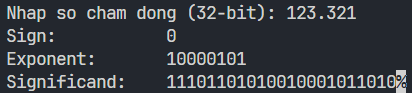
\includegraphics[width=0.875\textwidth]{imgs/1.png}
	\caption{Kết quả bài tập 1}
\end{figure}

\subsection{Bài 2}
\begin{figure}[!ht]
	\centering
	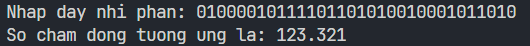
\includegraphics[width=0.875\linewidth]{imgs/2.png}
	\caption{Kết quả bài tập 2}
\end{figure}

\subsection{Bài 3}
\begin{figure}[!ht]
	\centering
	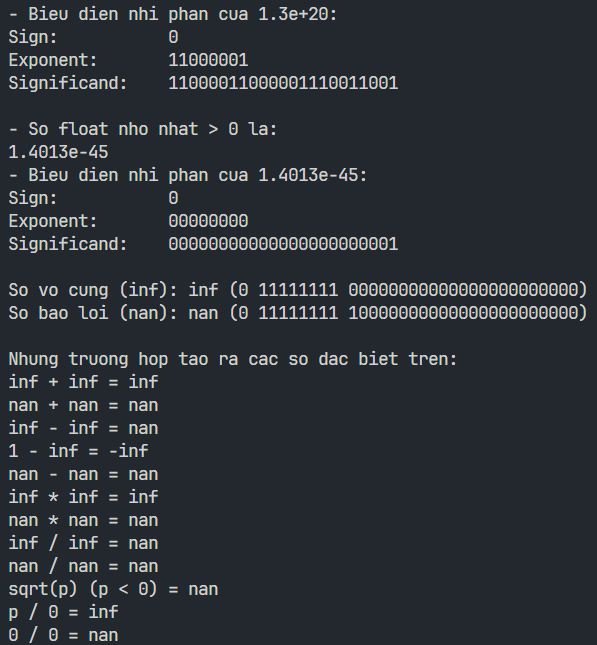
\includegraphics[width=0.7\linewidth]{imgs/3.png}
	\caption{Kết quả bài tập 3}
\end{figure}
\begin{flushleft}
	\textbf{Giải thích kết quả bài tập 3:}
	\begin{itemize}
		\item \textbf{inf + inf = inf}: Kết quả là \textbf{inf} vì khi cộng 2 số vô cùng, kết quả vẫn là vô cùng.
		\item \textbf{nan + nan = nan}: Kết quả là \textbf{nan} vì khi cộng 2 số không xác định, kết quả cũng không xác định.
		\item \textbf{inf - inf = nan}: Kết quả là \textbf{nan} vì khi trừ 2 số vô cùng, kết quả không xác định.
		\item \textbf{1 - inf = -inf}: Kết quả là \textbf{-inf} vì khi trừ một số hữu hạn với vô cùng, kết quả là vô cùng âm.
		\item \textbf{nan - nan = nan}: Kết quả là \textbf{nan} vì khi trừ 2 số không xác định, kết quả cũng không xác định.
		\item \textbf{inf * inf = inf}: Kết quả là \textbf{inf} vì khi nhân 2 số vô cùng, kết quả vẫn là vô cùng.
		\item \textbf{nan * nan = nan}: Kết quả là \textbf{nan} vì khi nhân 2 số không xác định, kết quả cũng không xác định.
		\item \textbf{inf / inf = nan}: Kết quả là \textbf{nan} vì khi chia 2 số vô cùng, kết quả không xác định.
		\item \textbf{nan / nan = nan}: Kết quả là \textbf{nan} vì khi chia 2 số không xác định, kết quả cũng không xác định.
		\item \textbf{sqrt(p) = nan (p < 0)}: Kết quả là \textbf{nan} vì căn bậc 2 của số âm không xác định.
		\item \textbf{p / 0 = inf}: Kết quả là \textbf{inf} vì khi chia một số hữu hạn cho 0, kết quả là vô cùng.
		\item \textbf{0 / 0 = nan}: Kết quả là \textbf{nan} vì khi chia 0 cho 0, kết quả không xác định.
	\end{itemize}
\end{flushleft}

\subsection{Bài 4}
\begin{figure}[!ht]
	\centering
	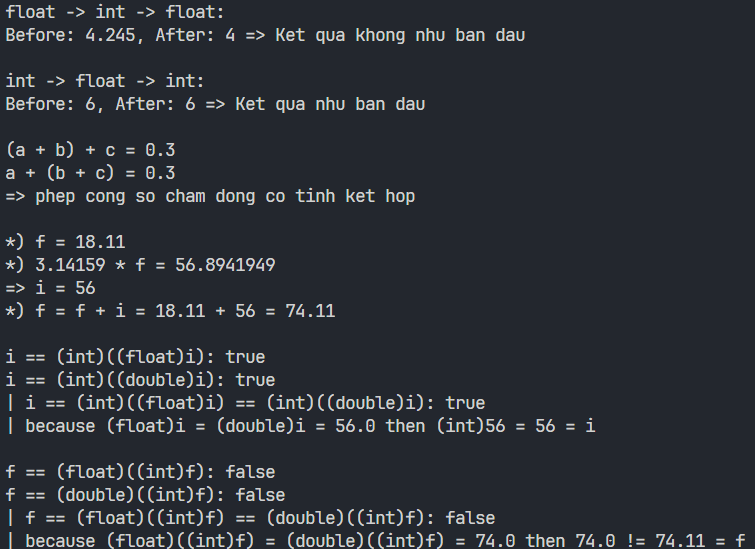
\includegraphics[width=0.7\linewidth]{imgs/4.png}
	\caption{Kết quả bài tập 4}
\end{figure}

\end{document}